\documentclass[aspectratio=169,11pt]{beamer}
\usetheme{Madrid}
\usecolortheme{whale}
\usepackage[utf8]{inputenc}
\usepackage[T1]{fontenc}
\usepackage[english]{babel}
\usepackage{graphicx}
\usepackage{tikz}
\usetikzlibrary{shapes.geometric,arrows.meta,positioning,calc,fit,backgrounds}
\usepackage{listings}
\usepackage{booktabs}

\definecolor{cblue}{HTML}{2c7fb8}
\definecolor{corange}{HTML}{f47216}
\definecolor{cgreen}{HTML}{2a9d4e}
\definecolor{cgray}{HTML}{555555}
\definecolor{codebg}{HTML}{f6f8fa}
\setbeamercolor{structure}{fg=cblue}
\setbeamertemplate{navigation symbols}{}

\lstdefinestyle{code}{
  backgroundcolor=\color{codebg}, basicstyle=\ttfamily\tiny,
  breaklines=true, keywordstyle=\color{cblue}\bfseries,
  commentstyle=\color{cgreen}\itshape, stringstyle=\color{corange},
  showstringspaces=false, columns=fullflexible}
\lstset{style=code}

\title[Distributed AI Recognition + Raft]{Distributed Object-Recognition System\\with AI and the Raft Consensus Algorithm}
\subtitle{CC4P1 -- Concurrent and Distributed Programming -- Final 2026-I}
\author[Iman, Ortega]{Melissa Iman Noriega \and Junior Ortega}
\institute[UNI-FC]{School of Computer Science -- Faculty of Sciences -- UNI}
\date{2026-I}

\begin{document}

\begin{frame}[plain]\titlepage\end{frame}

% ------------------------------------------------------------------
\begin{frame}{Outline}
\tableofcontents
\end{frame}

% ==================================================================
\section{Problem and requirements}

\begin{frame}{The problem}
\textbf{Goal:} a distributed system that recognizes objects (or animals/people)
with a previously trained AI model, and stays consistent and fault-tolerant
using the \textbf{Raft consensus algorithm}.
\vspace{0.4em}
\begin{itemize}
  \item \textbf{Training Server} -- trains the model and its weights; the load can
  be split across nodes (CPU-parallel). Weights are persisted.
  \item \textbf{Testing Server} -- each camera uses the trained model, recognizes
  objects on its own, stores an image and records the detection.
  \item \textbf{Watcher Client} -- shows the consistent detection log
  (type, camera, date/time).
  \item \textbf{Raft Consensus Module} -- replicated log + state machine; if a node
  fails, the others keep going.
\end{itemize}
\end{frame}

\begin{frame}{Hard constraints from the assignment}
\begin{itemize}
  \item \textbf{Raw native sockets only.} No WebSocket, Socket.IO, frameworks,
  RabbitMQ/MQ, or communication libraries. \textbf{Raft is implemented by hand over TCP.}
  \item \textbf{Three languages}, one node per student:
  \textbf{Java}, \textbf{Python}, \textbf{Go}.
  \item \textbf{Two operating systems} running the same set of languages.
  \item \textbf{Threads} for performance and to avoid record corruption.
  \item \textbf{Local deployment, no internet}, on LAN and WiFi.
  \item Only the base libraries of each language (NumPy allowed for the CNN).
\end{itemize}
\end{frame}

\begin{frame}{Team and languages}
\begin{center}
\begin{tabular}{@{}lll@{}}
\toprule
\textbf{Member} & \textbf{Language} & \textbf{Component} \\
\midrule
Melissa Iman & Java   & Raft core + distributed training + Watcher UI \\
Junior Ortega & Go    & Raft node + record state machine \\
(Python part) & Python & CNN + Testing Server + Raft node \\
\bottomrule
\end{tabular}
\end{center}
\vspace{0.6em}
All three nodes speak the \textbf{same text protocol}, so they form one
heterogeneous cluster.
\end{frame}

% ==================================================================
\section{Architecture}

\begin{frame}{System architecture}
\begin{center}
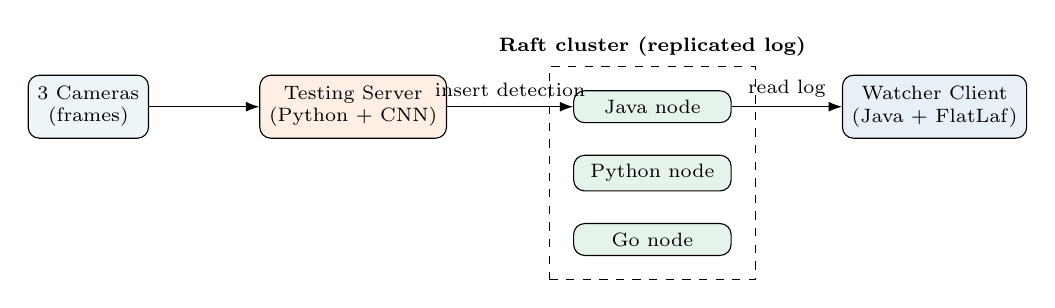
\begin{tikzpicture}[font=\scriptsize,>=Latex,node distance=6mm]
  \tikzstyle{box}=[draw,rounded corners,align=center,minimum height=8mm,fill=cblue!8]
  \tikzstyle{node3}=[draw,rounded corners,align=center,minimum width=20mm,fill=cgreen!12]

  % cameras
  \node[box] (cam) {3 Cameras\\(frames)};
  % testing server
  \node[box,right=14mm of cam,fill=corange!12] (test) {Testing Server\\(Python + CNN)};
  % cluster
  \node[node3,right=16mm of test] (java) {Java node};
  \node[node3,below=4mm of java] (py) {Python node};
  \node[node3,below=4mm of py] (go) {Go node};
  \node[draw,dashed,fit=(java)(py)(go),inner sep=3mm,label=above:{\textbf{Raft cluster (replicated log)}}] (clu) {};
  % watcher
  \node[box,right=14mm of java,fill=cblue!12] (watch) {Watcher Client\\(Java + FlatLaf)};

  \draw[->] (cam) -- (test);
  \draw[->] (test) -- node[above,sloped]{insert detection} (java.west);
  \draw[<-] (watch) -- node[above,sloped]{read log} (java.east);
\end{tikzpicture}
\end{center}
\begin{itemize}\scriptsize
  \item Cameras feed frames to the Testing Server; the CNN recognizes and inserts
  each detection into the cluster \textbf{through the leader}.
  \item The Watcher reads the committed, replicated log.
\end{itemize}
\end{frame}

% ==================================================================
\section{Raft consensus}

\begin{frame}{Raft: leader election and log replication}
\begin{columns}
\begin{column}{0.52\textwidth}
\textbf{States:} Follower / Candidate / Leader.
\begin{itemize}\scriptsize
  \item Randomized election timeout \textbf{150--300\,ms} (avoids split votes).
  \item \texttt{RequestVote} with the election restriction (candidate log must be
  up to date).
  \item \texttt{AppendEntries} replicates; an entry is \textbf{committed} once it is
  on a \textbf{majority}.
  \item Log Matching + \texttt{nextIndex} to repair followers.
  \item Only current-term entries commit by counting replicas.
\end{itemize}
\end{column}
\begin{column}{0.48\textwidth}
\begin{center}
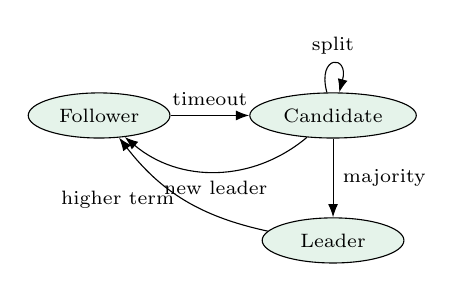
\begin{tikzpicture}[font=\scriptsize,>=Latex,node distance=10mm]
  \tikzstyle{s}=[draw,ellipse,fill=cgreen!12,minimum width=18mm]
  \node[s] (f) {Follower};
  \node[s,right=of f] (c) {Candidate};
  \node[s,below=of c] (l) {Leader};
  \draw[->] (f) -- node[above]{timeout} (c);
  \draw[->] (c) -- node[right]{majority} (l);
  \draw[->] (c) to[loop above] node{split} (c);
  \draw[->] (l) to[bend left=20] node[left]{higher term} (f);
  \draw[->] (c) to[bend left=40] node[below,sloped]{new leader} (f);
\end{tikzpicture}
\end{center}
\end{column}
\end{columns}
\end{frame}

\begin{frame}[fragile]{The text protocol (shared by the 3 languages)}
\footnotesize
One message per line, fields separated by \texttt{|}:
\begin{lstlisting}
REQUEST_VOTE|term|candidateId|lastLogIndex|lastLogTerm
VOTE|term|granted(1/0)
APPEND|term|leaderId|prevLogIndex|prevLogTerm|commitIndex|entries
APPEND_OK|term|success(1/0)|matchIndex

NUEVA_DETECCION|type,imageRef,dateTime,camera   -> insert a detection
LEER_REGISTRO                                    -> read the whole log
REGISTRO|det1;det2;det3;...                       -> reply to the Watcher
REDIRECT|leaderHost:leaderPort                    -> if a follower was contacted
OK                                                -> insertion accepted
\end{lstlisting}
Because Java, Python and Go all use this exact format, a node in any language
interoperates with the others.
\end{frame}

% ==================================================================
\section{AI model}

\begin{frame}{The CNN (from scratch with NumPy)}
\begin{columns}
\begin{column}{0.55\textwidth}
\textbf{Architecture} (5 classes of figures):
\begin{center}\scriptsize
input $1\times28\times28$\\
$\downarrow$ Conv 8@3x3 + ReLU + MaxPool\\
$\downarrow$ Conv 16@3x3 + ReLU + MaxPool\\
$\downarrow$ Flatten + Dense + Softmax
\end{center}
\begin{itemize}\scriptsize
  \item Full forward + backward (real backprop), convolution via im2col.
  \item No TensorFlow/PyTorch -- only NumPy, works offline.
  \item Weights persisted to disk (\texttt{.npz}).
\end{itemize}
\end{column}
\begin{column}{0.45\textwidth}
\textbf{Distributed training}
\begin{itemize}\scriptsize
  \item Data-parallel: each mini-batch is split into shards, one worker per shard,
  gradients are averaged (all-reduce).
  \item \texttt{multiprocessing} (real CPU parallelism, avoids the GIL).
\end{itemize}
\vspace{0.3em}
\begin{center}
\textbf{97.2\%} test accuracy\\
same result, faster (4.7s vs 11s)
\end{center}
\end{column}
\end{columns}
\end{frame}

% ==================================================================
\section{Results and demo}

\begin{frame}{End-to-end: heterogeneous cluster}
\textbf{Verified} with the three languages running together:
\begin{itemize}
  \item Java + Python + Go elect a leader among themselves and replicate.
  \item The Testing Server runs the CNN on 3 cameras (one thread each) and inserts
  detections into the cluster.
  \item \textbf{All three nodes apply the same 75 detections in the same order.}
\end{itemize}
\vspace{0.3em}
\begin{center}\footnotesize
\begin{tabular}{@{}lccc@{}}
\toprule
& Java & Python & Go \\
\midrule
applied entries & 75 & 75 & 75 \\
\bottomrule
\end{tabular}
\end{center}
\end{frame}

\begin{frame}{Fault tolerance (leader failover)}
\begin{itemize}
  \item With Python as leader, we kill it mid-run.
  \item \textbf{Go is re-elected} leader in the next term.
  \item Previous detections survive: the log stays consistent.
  \item Inserting through the new leader keeps working.
\end{itemize}
\vspace{0.5em}
\begin{center}\itshape
"If a node fails, the others keep going and the record stays consistent." -- exactly
what the assignment asks for.
\end{center}
\end{frame}

\begin{frame}{Recognition -- real detections from the CNN}
\begin{center}
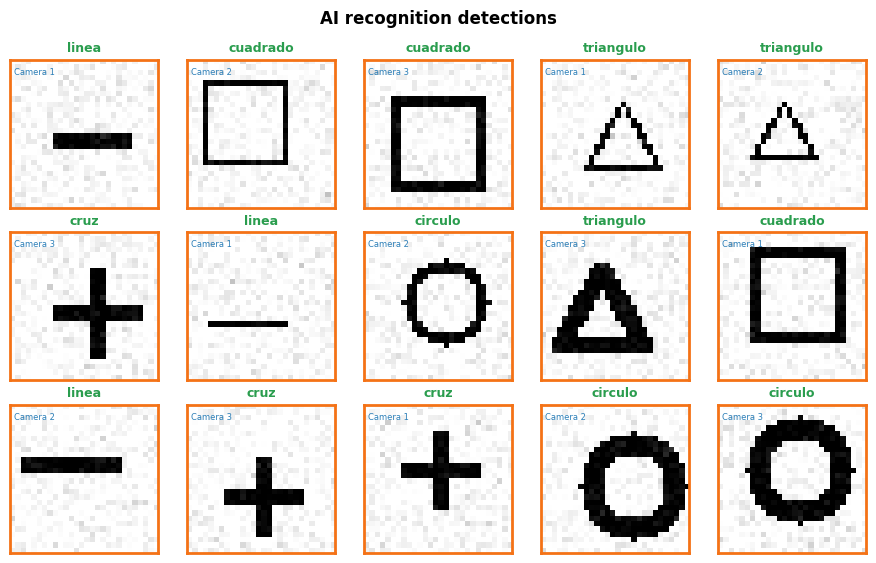
\includegraphics[width=0.82\textwidth]{../img/hoja_detecciones.png}
\end{center}
\vspace{-0.3em}
{\scriptsize Each frame is recognized by the trained CNN (label in green, camera in
blue). These are the images the Testing Server stores for every detection.}
\end{frame}

\begin{frame}{Watcher Client -- live replicated log}
% TODO SCREENSHOT: aqui va el screenshot del Vigilante (UI Java+FlatLaf) conectado
% al cluster, mostrando la tabla de detecciones en vivo. Reemplazar el recuadro.
\begin{center}
\fbox{\parbox{0.75\textwidth}{\centering\vspace{2.2cm}
\textbf{[ screenshot: Watcher UI showing the live detection log }\\
\textbf{(type, camera, date/time) while the cluster runs ]}
\vspace{2.2cm}}}
\end{center}
{\scriptsize The Watcher reads the committed log from the leader and refreshes
every second.}
\end{frame}

\begin{frame}{Compliance with the constraints}
\footnotesize
\begin{tabular}{@{}ll@{}}
\toprule
\textbf{Requirement} & \textbf{Status} \\
\midrule
Raw native sockets only (no frameworks/MQ) & Done -- Raft by hand over TCP \\
Three languages, one node each & Done -- Java / Python / Go \\
Threads for performance / no corruption & Done -- threads, goroutines, mutex \\
Previously trained AI + persisted weights & Done -- CNN 97.2\%, \texttt{.npz} \\
Distributed CPU-parallel training & Done -- multiprocessing all-reduce \\
$\geq 3$ cameras & Done -- 3 camera threads \\
Fault tolerance (Raft) & Done -- verified failover \\
LAN/WiFi, 2 OS & Pending for the live demo \\
\bottomrule
\end{tabular}
\end{frame}

\begin{frame}[plain]
\begin{center}
{\Large\textbf{Thank you}}\\[0.5em]
Distributed Object-Recognition System with AI and Raft\\
CC4P1 -- 2026-I
\end{center}
\end{frame}

\end{document}
